\section{Diseño del esquema de base de datos}
\label{sec:diseno_base_datos}

Para la capa de persistencia se ha seleccionado PostgreSQL 16 junto con el motor de migraciones Flyway. Todas las entidades emplean identificadores de tipo \texttt{UUID} generados de forma aleatoria (versión 4). La ventaja directa frente a secuencias autonuméricas clásicas radica en impedir que clientes maliciosos deduzcan volúmenes de usuarios, inmuebles o transacciones mediante peticiones consecutivas a la API REST.

El esquema completo consta de diecisiete tablas con restricciones foráneas explícitas y borrado lógico (\emph{soft delete}) en las entidades de mayor criticidad. Para facilitar la comprensión del modelo relacional, las tablas se agrupan a continuación en cuatro dominios operativos antes de presentar la vista integrada.

\subsection{Módulo de identidad, cuentas y seguridad}

El núcleo de usuarios se concentra en la tabla \texttt{users}. La definición recoge los datos personales habituales (\texttt{email}, \texttt{password} hasheada, \texttt{full\_name}, \texttt{phone} y \texttt{birth\_date}) y gestiona el control de acceso a través de la columna \texttt{role}, que almacena roles del sistema como \texttt{ROLE\_USER} o \texttt{ROLE\_ADMIN}.

\begin{figure}[H]
    \centering
    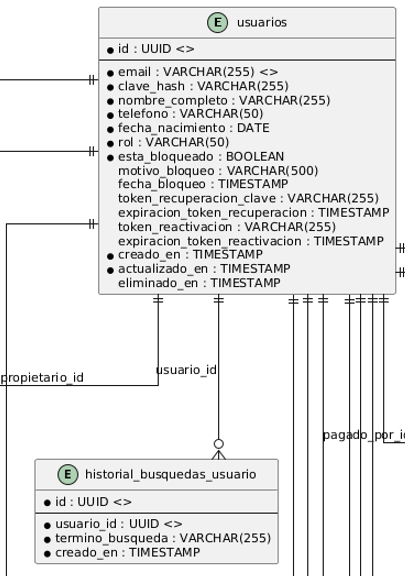
\includegraphics[width=0.75\textwidth]{AnalisisFuncional/img/db_part1_users.png}
    \caption{Esquema relacional: Usuarios y registros de búsqueda}
    \label{fig:db_part1_users}
\end{figure}

El ciclo de vida de la cuenta incorpora medidas frente a bloqueos administrativos y recuperaciones seguras:
\begin{itemize}
    \item \textbf{Gestión de suspensiones:} Los campos \texttt{is\_banned}, \texttt{banned\_reason} y \texttt{banned\_at} permiten a los administradores inhabilitar el inicio de sesión manteniendo el histórico de auditoría intacto.
    \item \textbf{Tókenes con tiempo de expiración:} Se separan los tókenes de restablecimiento de contraseña (\texttt{password\_reset\_token}) de los de reactivación voluntaria (\texttt{reactivation\_token}), ambos acompañados por su correspondiente marca temporal de caducidad (\texttt{*\_expires\_at}). Gracias a los índices añadidos en la migración \texttt{V19}, el cron \texttt{UserTokenCleanupTask} purga periódicamente las claves vencidas.
    \item \textbf{Borrado lógico:} La columna \texttt{deleted\_at} marca cuentas dadas de baja sin romper restricciones foráneas en contratos de reserva pasados o historiales de gastos.
\end{itemize}

A este bloque se vincula la tabla \texttt{user\_search\_history}, que guarda los términos de búsqueda introducidos en el explorador junto a una referencia \texttt{user\_id}. Este registro permite al servicio \texttt{RecommendationServiceImpl} inferir ciudades de interés y ofrecer anuncios relevantes.

\subsection{Módulo inmobiliario, catálogo y reservas}

Este subsistema separa la propiedad física del anuncio comercial para dar soporte a viviendas completas y a habitaciones independientes dentro del mismo inmueble.

\begin{figure}[H]
    \centering
    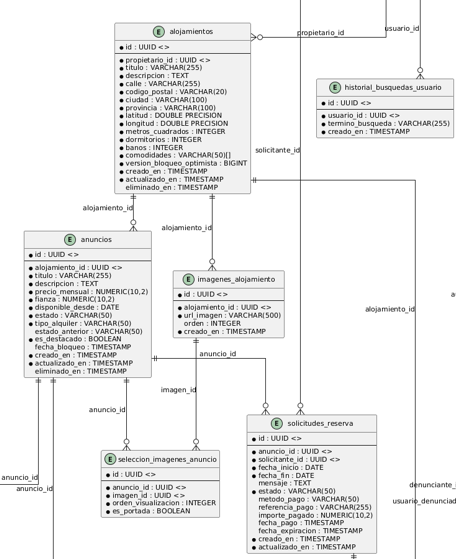
\includegraphics[width=0.95\textwidth]{AnalisisFuncional/img/db_part2_housing.png}
    \caption{Esquema relacional: Parque inmobiliario, publicaciones y reservas}
    \label{fig:db_part2_housing}
\end{figure}

\subsubsection{Estructura del alojamiento e imágenes}
La tabla \texttt{accommodations} describe la finca registral o vivienda base: dirección postal, coordenadas espaciales (\texttt{latitude}, \texttt{longitude}), distribución física (\texttt{bedrooms}, \texttt{bathrooms}, \texttt{square\_meters}) y un array nativo de PostgreSQL (\texttt{amenities}) para servicios como ascensor o calefacción. Incorpora la columna \texttt{version} para implementar control de concurrencia optimista y evitar que dos peticiones simultáneas sobreescriban modificaciones concurrentes.

Las fotos subidas a Cloudinary se guardan en \texttt{accommodation\_images}, enlazadas por \texttt{accommodation\_id} con un \texttt{order\_index} para la galería general de la propiedad.

\subsubsection{Publicaciones y selección multimedia}
Para comercializar estancias se utiliza \texttt{accommodation\_listings}. Cada fila apunta a su \texttt{accommodation\_id} y define las condiciones económicas: \texttt{price\_per\_month}, \texttt{security\_deposit}, \texttt{available\_from}, \texttt{rental\_type} (piso completo o habitación) y \texttt{status} (\texttt{DRAFT}, \texttt{ACTIVE}, \texttt{PAUSED}, \texttt{BANNED}). El flag booleano \texttt{is\_promoted} prioriza el anuncio en los algoritmos de recomendación.

Dado que un anfitrión puede alquilar habitaciones individuales del mismo piso, no todas las imágenes de la vivienda aplican a un anuncio concreto. La tabla asociativa \texttt{listing\_image\_selection} resuelve este desacoplamiento: relaciona \texttt{listing\_id} con \texttt{image\_id}, añadiendo \texttt{display\_order} y un booleano \texttt{is\_cover} para designar la portada de cada publicación.

\subsubsection{Contratación y evaluaciones}
La gestión de estancias recae en \texttt{booking\_requests}. Conecta al inquilino (\texttt{requester\_id}) con el anuncio (\texttt{listing\_id}) mediante un intervalo cerrado (\texttt{start\_date}, \texttt{end\_date}). Incluye los campos \texttt{amount\_paid}, \texttt{payment\_method}, \texttt{payment\_reference} y \texttt{paid\_at} para registrar el cobro de la fianza gestionado por \texttt{PaymentService}. El campo \texttt{expires\_at} permite cancelar automáticamente solicitudes desatendidas por el anfitrión mediante la tarea programada \texttt{BookingExpirationTask}.

Cuando la estancia concluye, el inquilino puede puntuar el alojamiento en \texttt{accommodation\_reviews}. Para garantizar que solo opinen personas que realmente se han hospedado, la tabla establece una restricción de unicidad sobre la clave foránea \texttt{booking\_request\_id}, evitando valoraciones duplicadas o no verificadas sobre la propiedad.

\subsection{Módulo de convivencia doméstica, finanzas y tareas}

El bloque de gestión de piso compartido resuelve las dinámicas internas de convivencia entre compañeros.

\begin{figure}[H]
    \centering
    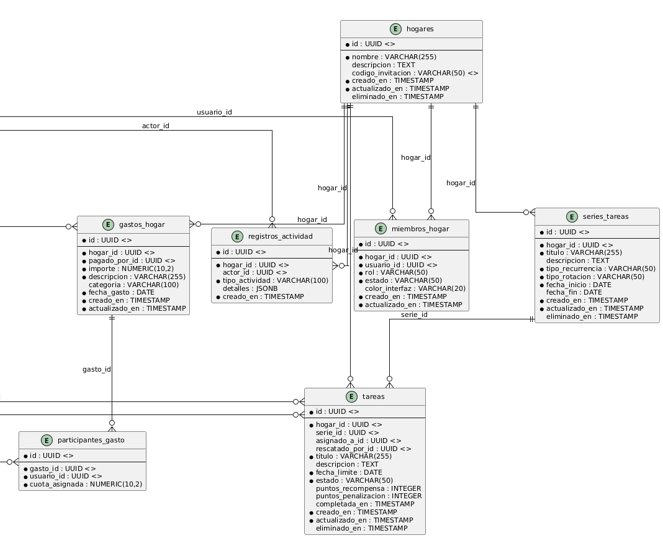
\includegraphics[width=0.95\textwidth]{AnalisisFuncional/img/db_part3_living.png}
    \caption{Esquema relacional: Convivencia, reparto de gastos y cuadrante de tareas}
    \label{fig:db_part3_living}
\end{figure}

\subsubsection{Espacio del hogar y membresías}
La tabla \texttt{homes} representa la comunidad doméstica. Contiene el nombre del grupo y la columna \texttt{invitation\_code}, marcada como única, que almacena las claves temporales generadas por \texttt{InvitationCodeGenerator} para invitar a nuevos integrantes.

La pertenencia se gestiona en \texttt{home\_members}. Cada fila asocia un usuario con un hogar, indicando su rol (\texttt{ADMIN} o \texttt{MEMBER}) y su estado (\texttt{ACTIVE}, \texttt{LEFT}, \texttt{EXPELLED}). Se incluye un campo \texttt{color} con el valor hexadecimal elegido por el compañero para teñir sus turnos en el calendario.

\subsubsection{Motor contable y reparto de costes}
El subsistema de gastos se compone de dos tablas con relación uno a muchos:
\begin{itemize}
    \item \texttt{home\_expenses}: Registra la cabecera del pago realizado dentro del hogar (\texttt{home\_id}), el pagador (\texttt{paid\_by\_id}), el importe total (\texttt{amount}), la fecha y el concepto.
    \item \texttt{home\_expense\_participants}: Desglosa la deuda individual. Cada registro vincula el gasto (\texttt{expense\_id}) con un miembro del hogar (\texttt{user\_id}) y almacena su cuota exacta (\texttt{share\_amount}).
\end{itemize}
Esta separación proporciona las entradas necesarias para que \texttt{DebtSimplifierService} cruce débitos y créditos, minimizando las transferencias requeridas para saldar cuentas.

\subsubsection{Cuadrante recurrente y gamificación de tareas}
La organización de limpiezas y compras se apoya en dos entidades complementarias:
\begin{itemize}
    \item \texttt{chore\_series}: Modela la regla recurrente configurada por el administrador. Define la periodicidad (\texttt{DAILY}, \texttt{WEEKLY}, \texttt{MONTHLY}) y la estrategia de asignación (\texttt{FIXED} o \texttt{ROUND\_ROBIN}).
    \item \texttt{chores}: Representa la tarea individual con fecha límite (\texttt{due\_date}). Mantiene la clave foránea opcional \texttt{series\_id} si proviene de un ciclo repetitivo, el responsable inicial (\texttt{assigned\_to\_id}) y las columnas de gamificación: \texttt{points\_reward}, \texttt{points\_penalty} y \texttt{rescued\_by\_id}. Cuando una tarea entra en estado \texttt{OVERDUE}, cualquier miembro puede completarla y adjudicarse los puntos de rescate.
\end{itemize}

\subsection{Módulo de mensajería, auditoría y moderación}

El último dominio comprende las herramientas de comunicación interpersonal y las pistas de auditoría del sistema.

\begin{figure}[H]
    \centering
    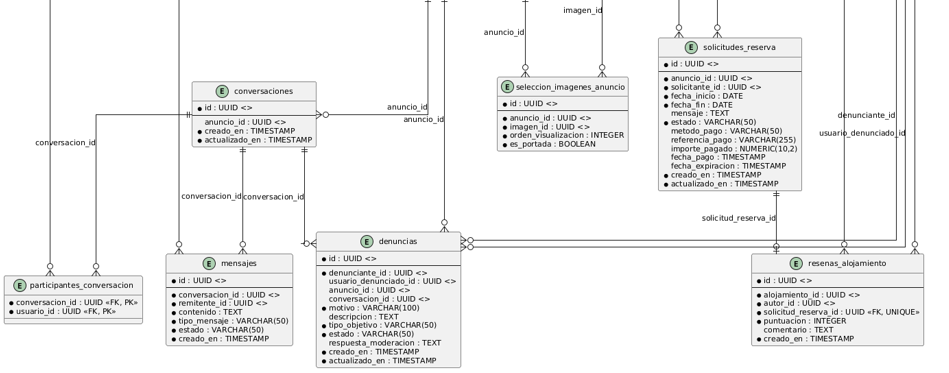
\includegraphics[width=0.85\textwidth]{AnalisisFuncional/img/db_part4_support.png}
    \caption{Esquema relacional: Mensajería directa, auditoría y denuncias}
    \label{fig:db_part4_support}
\end{figure}

\subsubsection{Canal de chat contextual}
Las conversaciones se estructuran en \texttt{conversations}, con una referencia opcional al anuncio en negociación (\texttt{listing\_id}). Los participantes se normalizan a través de la tabla intermedia asociativa \texttt{conversation\_participants}. 

Cada mensaje individual se almacena en \texttt{messages}, enlazando la conversación (\texttt{conversation\_id}) y el remitente (\texttt{sender\_id}). La columna \texttt{message\_type} permite distinguir mensajes de texto estándar redactados por inquilinos o anfitriones de notificaciones automáticas del sistema generadas por eventos de reserva.

\subsubsection{Trazabilidad y muro de actividad}
Para reflejar altas de usuarios, creación de gastos o resoluciones de tareas en el muro del piso, la tabla \texttt{activity\_logs} almacena eventos disparados dentro de un hogar. Dispone de \texttt{actor\_id} con soporte de valores nulos (para acciones ejecutadas por procesos batch o del sistema), el tipo de evento (\texttt{activity\_type}) y una columna \texttt{details} de tipo nativo \texttt{JSONB}. Esta elección permite persistir metadatos variables de cada evento sin obligar a continuas alteraciones del esquema en la base de datos relacional.

\subsubsection{Centro de moderación administrativa}
La tabla \texttt{reports} canaliza las denuncias de comportamientos ilícitos. Almacena al informante (\texttt{reporter\_id}), la tipología del objeto reportado (\texttt{target\_type}) y claves foráneas polimórficas opcionales hacia el usuario infractor (\texttt{reported\_user\_id}), el anuncio bajo sospecha (\texttt{listing\_id}) o el hilo de chat (\texttt{conversation\_id}). 

Cuando un moderador examina las evidencias y aplica una sanción, actualiza la columna \texttt{status} a \texttt{RESOLVED} o \texttt{DISMISSED} y registra sus observaciones en \texttt{feedback}, activando el envío del correo de resolución al usuario denunciante.

\subsection{Esquema Base de Datos integrado}

La figura \ref{fig:db_er_global} recopila la totalidad de tablas, claves primarias, claves foráneas y cardinalidades operativas que conforman el almacenamiento relacional de Colivi.

\begin{figure}[H]
    \centering
    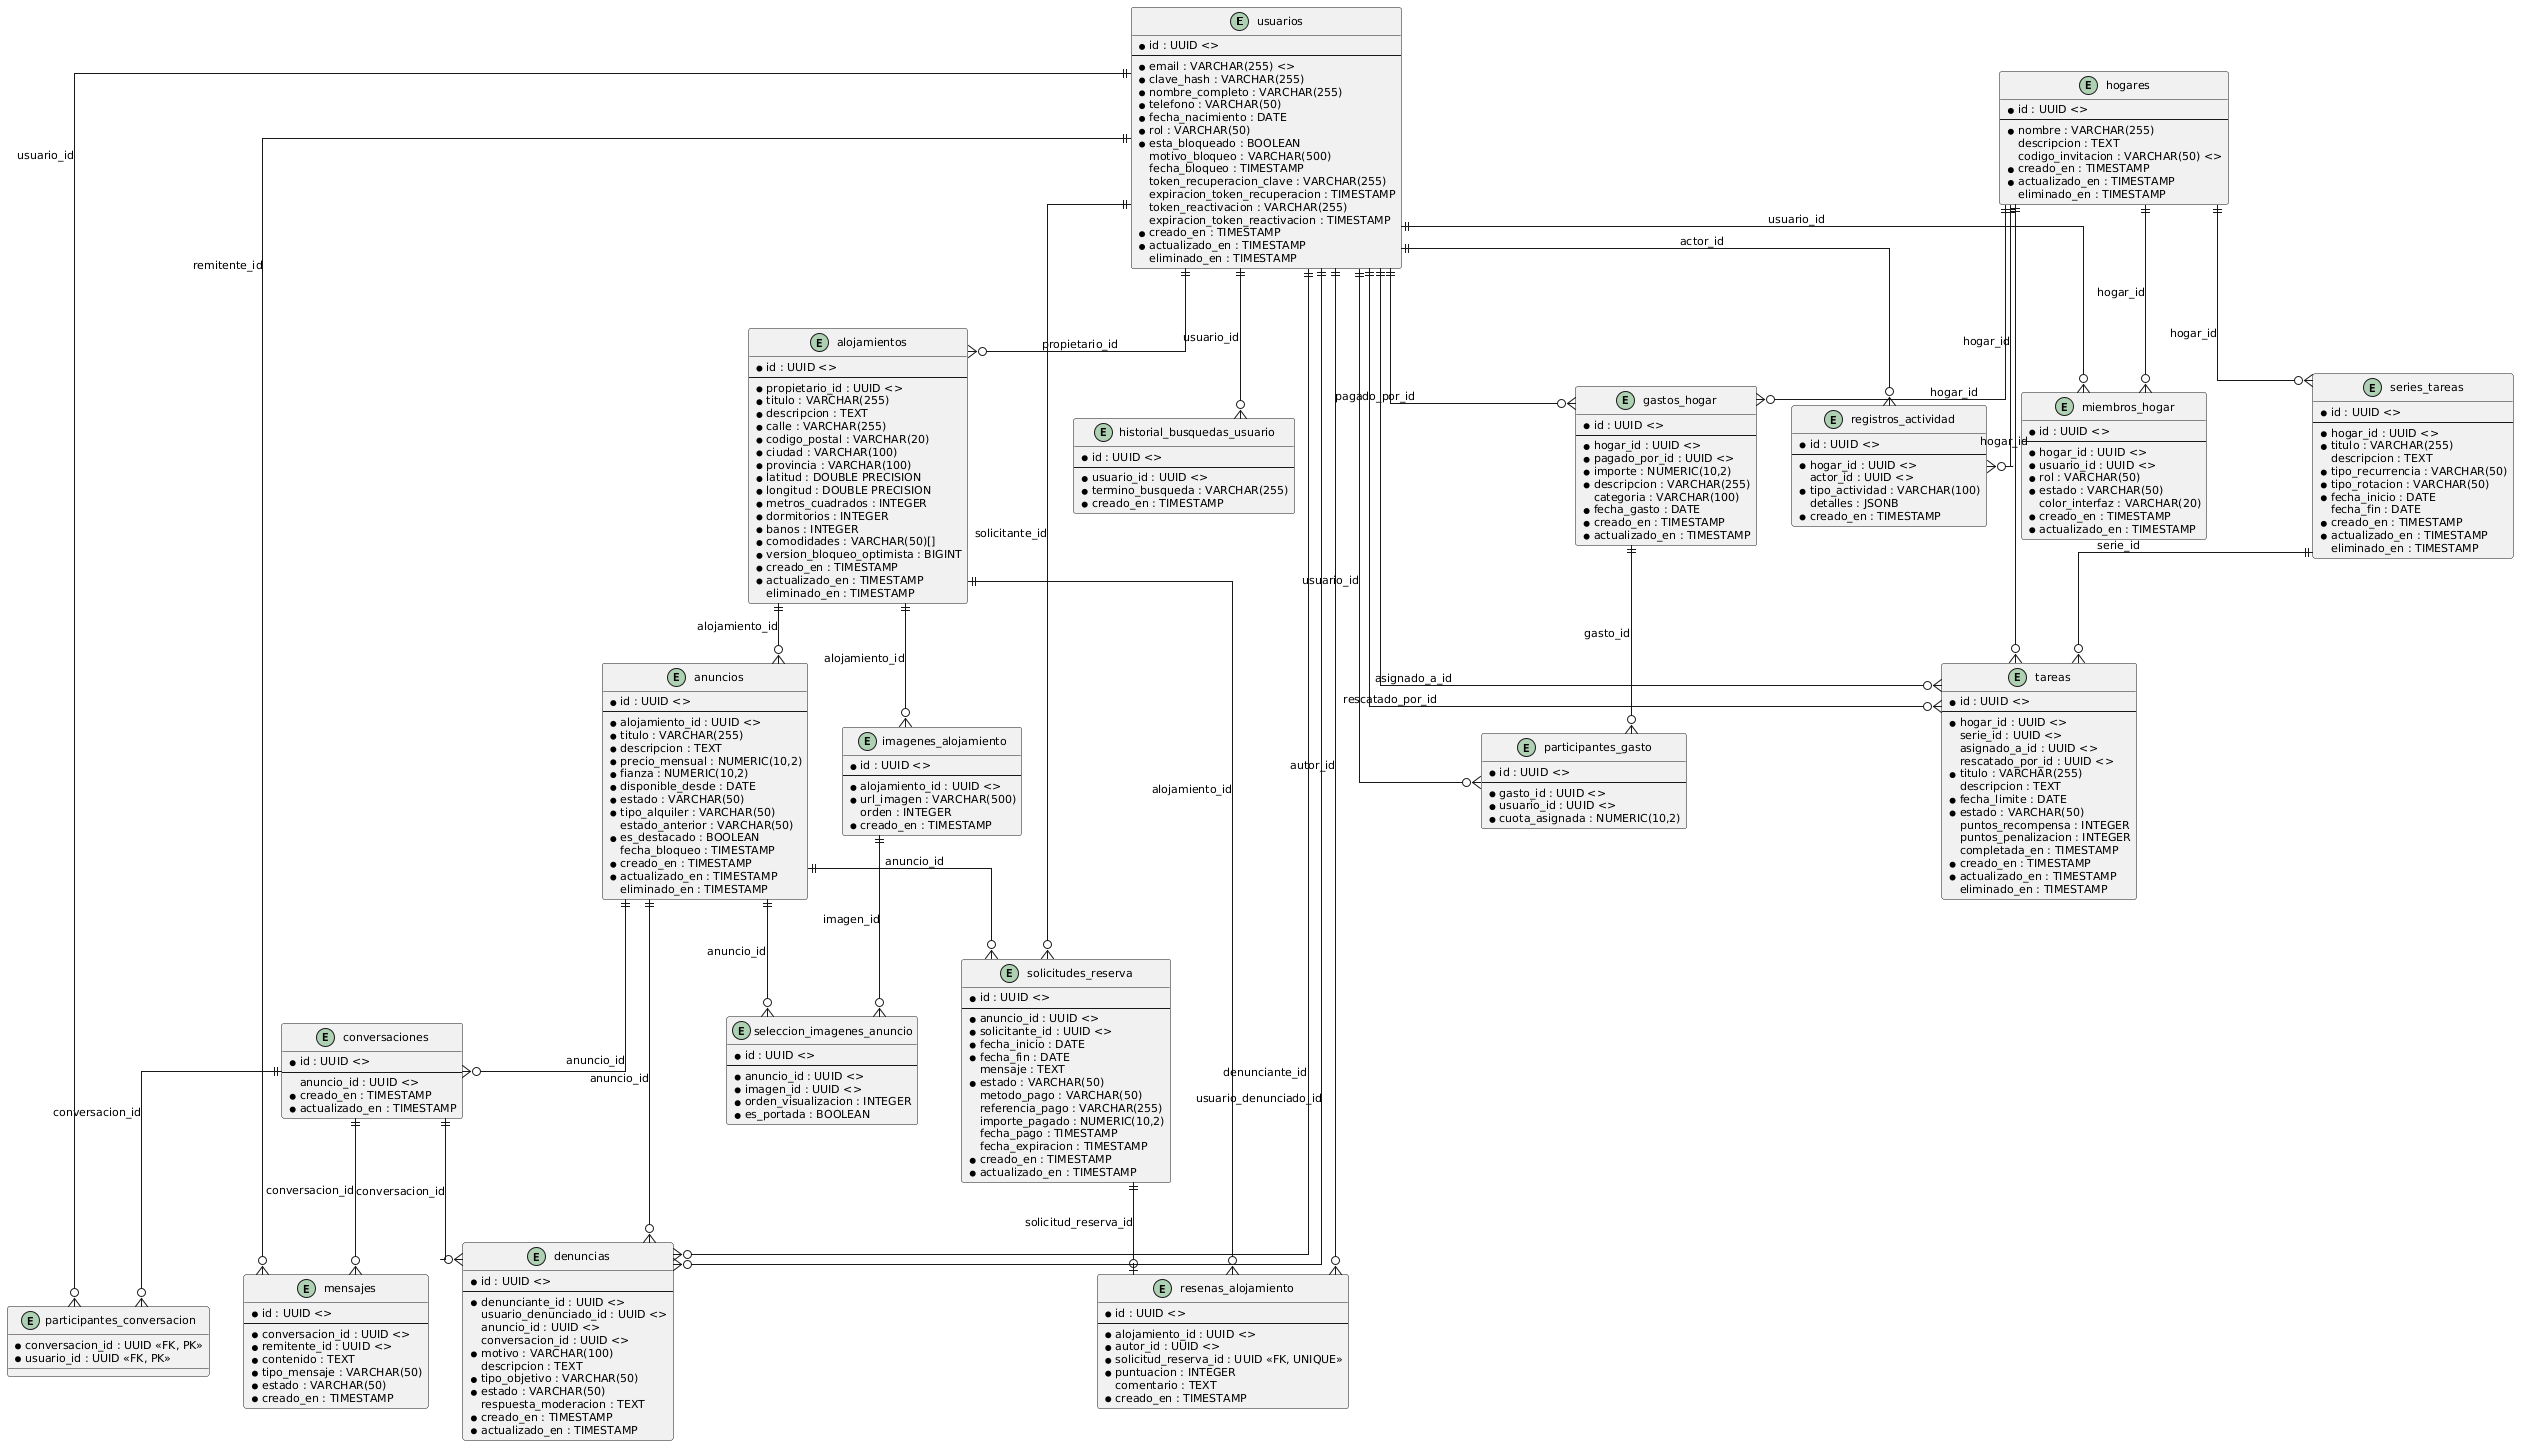
\includegraphics[width=\textwidth]{AnalisisFuncional/img/db_er_global.png}
    \caption{Diagrama de Base de Datos global del sistema Colivi}
    \label{fig:db_er_global}
\end{figure}